\documentclass[12pt]{article}

\usepackage[utf8]{inputenc}
\usepackage[T1]{fontenc}
\usepackage[spanish]{babel}
\usepackage{graphicx}
\usepackage{listings}
\usepackage{caption}
\usepackage{subcaption}
\usepackage[right=2cm,left=2cm,top=2cm,bottom=2cm]{geometry}
\usepackage{hyperref}
\usepackage{fancyhdr}
\usepackage{color}
\usepackage[export]{adjustbox}
\usepackage{graphicx}
\usepackage{float}
\usepackage{changepage}
\usepackage{multicol}
\usepackage{imakeidx}
\usepackage{csquotes}
\usepackage{array}
\usepackage{tabularx}
\usepackage{xcolor}
\usepackage[backend=biber]{biblatex}
\addbibresource{webgrafia.bib}

\pagestyle{fancy}
\renewcommand{\footrulewidth}{0.4pt}
\setlength{\headheight}{15pt}


\fancyhead[L]{ CEIABD – SBD }
\fancyhead[R]{ Páez Anguita, Víctor }
\fancyfoot[L]{IES Gran Capitán}


\begin{document}

\begin{titlepage}
    \begin{center}
      \Large \bfseries{}
    \end{center}
    \vspace{0.1cm}
    \begin{center}
      \Large \bfseries{}
    \end{center}
    \vspace{0.1cm}
    \begin{center}
     \Large \bfseries{Tipos de procesamiento en Big Data}
    \end{center}
    \vspace{0.0001cm}
    \begin{center}
        Departamento de informática \\ I.E.S. Gran Capitán - Córdoba
    \end{center}
        \vspace{2 cm}
\begin{figure}[h!]
    \centering
    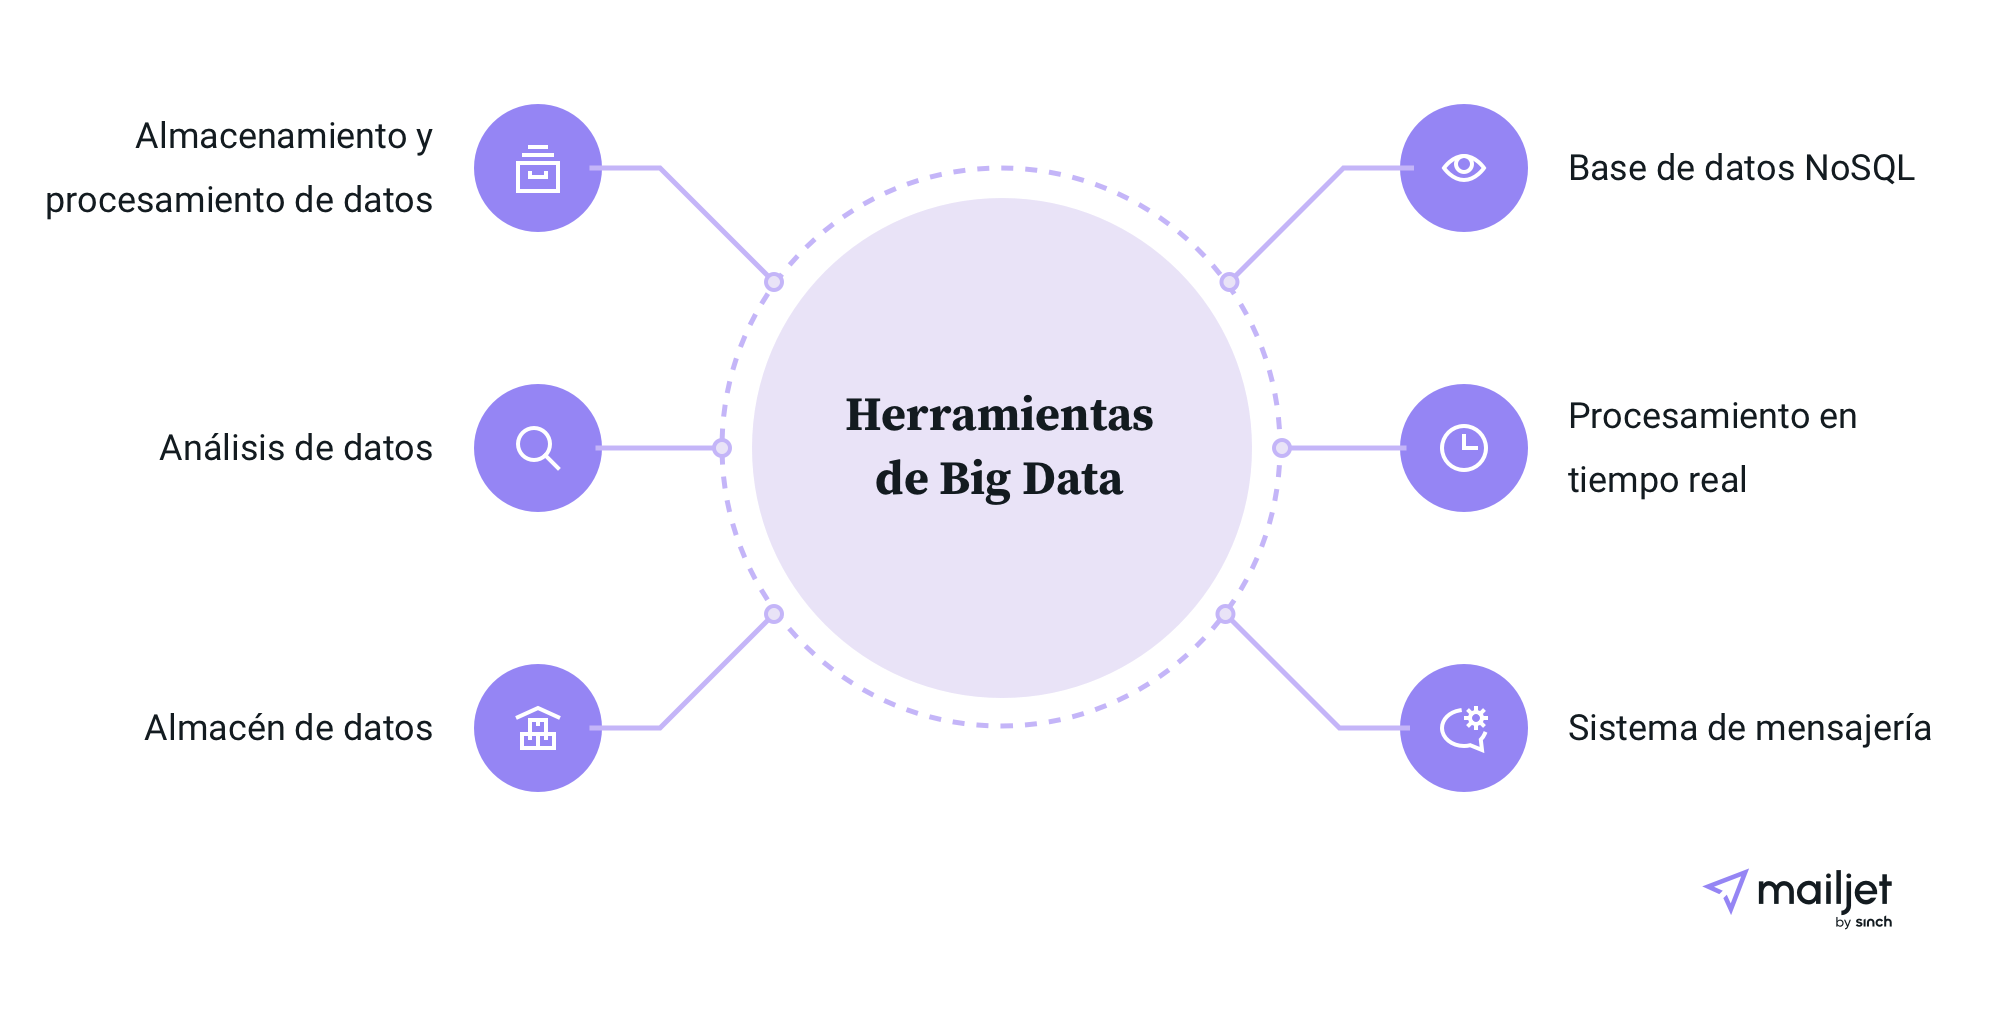
\includegraphics[width=.6\textwidth]{Portada.png}
    \label{fig:my_label}
\end{figure}
    \vspace{0.2 cm}
    \begin{center}
        Inteligencia artificial y Big data \\ Córdoba, 13 de Noviembre 2024
    \end{center}
    \vspace{4 cm}
\null\hfill \textbf{Desarrollado por:}
\\
\\
\null\hfill Víctor Páez Anguita
\clearpage
\end{titlepage}

%%%%%%%%%%%%%%%%%%%%%%%%%%%Index%%%%%%%%%%%%%%%%%%%%%%%%%%%%%%%%
\tableofcontents
\clearpage
%%%%%%%%%%%%%%%%%%%%%%%%%%%Index%%%%%%%%%%%%%%%%%%%%%%%%%%%%%%%%

\section{Introducción}

A continuación veremos los diferentes tipos de procesamiento de datos en Big Data. Cuales son, como funcionan, sus ventajas y desventajas
además de casos de usos de los mismos. Finalmente concluiremos con una tabla comparativa de estos.

\section{Procesamiento por Lotes (Batch)}

\subsection{Definición}

El procesamiento por lotes (batch) es un tipo de metodo que usan los ordenadores para completar grandes volumenes de tareas, llegando 
a ser ejecutado de manera simultanea o en orden secuencial sin parar. Este tipo de procesamiento se ejecuta sin la supervisión directa
del usuario.
\\
Este funciona de tal manera que el usuario introduce un conjunto de datos y una serie de parametros en un programa como puede ser (AWS), 
el cual se encarga de procesar los datos de manera automática.
\\
Este tipo de procesamiento es muy útil para tareas como la renderización de fotogramas para peliculas, para generar extractos bancarios,
para procesar nóminas, para realizar copias de seguridad, etc. Mayormente todo lo que requiera un gran volumen de datos y que no requiera
una respuesta inmediata.

\begin{figure}[h!]
    \centering
    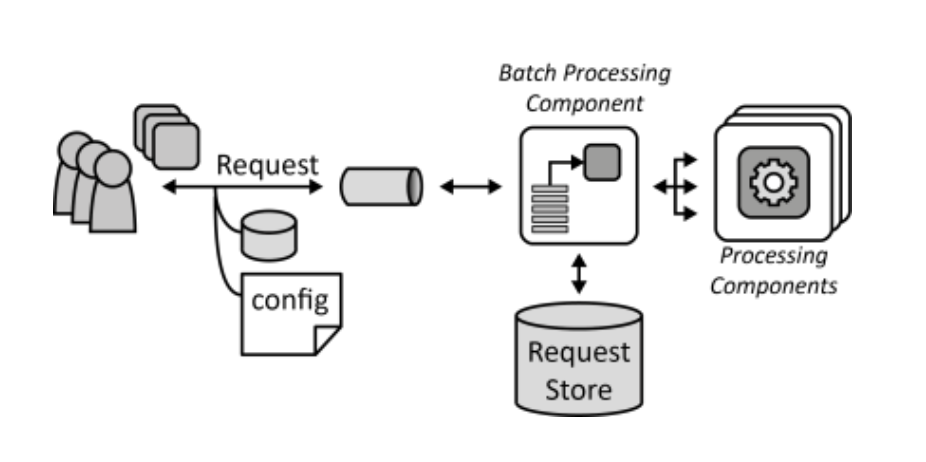
\includegraphics[width=.6\textwidth]{Batch.PNG}
    \label{fig:my_label}
\end{figure}

\subsection{Ejemplos}

\begin{itemize}
    \item \textbf{Servicios financieros}\\
    Este tipo de entidades han utilizado el procesamiento por lotes para la administración de riesgo, el procesamiento de transacciones al
    final del día y la vigilancia de fraudes.Utilizan el procesamiento por lotes para minimizar los errores humanos, aumentar la velocidad
    y la precisión, y reducir los costos con la automatización.

    \item \textbf{Software como servicio}\\
    Las empresas que brindan aplicaciones de software como servicio (SaaS) suelen enfrentar desafíos relacionados con la escalabilidad. 
    Implementar el procesamiento por lotes permite gestionar la creciente demanda de los clientes y automatizar la planificación de tareas. 

    \item \textbf{Investigación médica}\\
    El análisis de grandes volúmenes de datos en investigación es un requisito muy común. Por ejemplo, los científicos utilizan el 
    procesamiento por lotes para obtener mejores datos a fin de comenzar el diseño de fármacos y obtener una comprensión más profunda de 
    la función de un proceso bioquímico en particular. 

    \item \textbf{Medios digitales}\\
    Las empresas de medios y entretenimiento requieren sistemas de procesamiento por lotes altamente escalables para procesar datos 
    automáticamente, como archivos, gráficos y efectos visuales, para el contenido de video de alta resolución.
\end{itemize}

\subsection{Ventajas}

\begin{itemize}
    \item \textbf{Solución rápida y con coste menor}\\
    Debido a que la iteración del usuario sobre el proceso es mínima, ayuda a reducir el tiempo de ejecución y el coste de la operación. Tampoco
    requiere de hardware adicional para la ejecución de las tareas.
    \\ 
    No da posibilidad de errores humanos. Lo cual resulta en un proceso rápidoy preciso.

    \item \textbf{Características fuera de línea}\\
    El procesamiento por lotes se puede realizar en cualquier momento, esto permite que se pueda realizar en momentos de baja demanda de recursos.
    Se realizan en segundo plano, por lo que no afecta a la interacción del usuario.

    \item \textbf{Gestión sencilla y sin intervención de grandes procesos repetitivos}\\
    Facilita al usuario hacer su trabajo sin tener que preocuparse por la ejecución de tareas repetitivas. Si hay algún problema o error, se
    le notifica a la persona encargada.
\end{itemize}


\subsection{Desventajas}

\begin{itemize}
    \item \textbf{Despliegue y entrenamiento}\\
    Se debe de tener un nivel de conocimientos adecuado del manejo de estos sistemas. El usuario el cual no tenga conocimientos previos, deberá
    entender ciertos conceptos para poder realizar el procesamiento por lotes.

    \item \textbf{Coste}\\
    Si bien es cierto que el coste de ejecución es menor, el coste de implementación y mantenimiento puede ser elevado. Además de requerir como
    hemos descrito anteriormente, un nivel de conocimientos adecuado. Por lo que a pesar de ser una solución valiosa, es más factible para
    empresas grandes.

    \item \textbf{La depuración es difícil}\\
    La depuración de estos sistemas puede llegar a ser muy compleja, ya que se ejecutan en segundo plano y no se puede ver el proceso en tiempo
    real. Por lo que si hay algún error, puede ser complicado de encontrar. Se necesitará de un usuario con conocimientos.
\end{itemize}

\section{Procesamiento en Streaming}

\subsection{Definición}

El procesamiento en streaming es un método de procesamiento de datos en tiempo real (practicamente), en el que los datos se procesan a medida que 
se generan. Al usar tecnología para el procesamiento de streams, los streams de eventos se pueden almacenar, analizar, procesar e incluso actuar 
sobre ellos en tiempo real a medida que se generan.
\\
Este tipo de procesamiento implica la recopilación y el análisis de datos en tiempo real. Contiene tres tipos de componentes principales:

\begin{itemize}
    \item \textbf{Productores de secuencias}\\
    recopilan y envían datos a un procesador de secuencias, que agrupa temporalmente los registros por nombre y número de secuencia 
    para su procesamiento cronológico.
    \item \textbf{Consumidores de secuencias}\\
    procesan estos datos utilizando técnicas como agregación, filtros o machine learning, y pueden generar nuevas secuencias o devolver 
    los datos modificados al procesador.
\end{itemize}

A diferencia del procesamiento por lotes, el procesamiento en streaming permite analizar y actuar sobre los datos en tiempo real, pero solo
maneja registros individuales o micro batches con flujos de datos infinitos. 

\begin{figure}[h!]
    \centering
    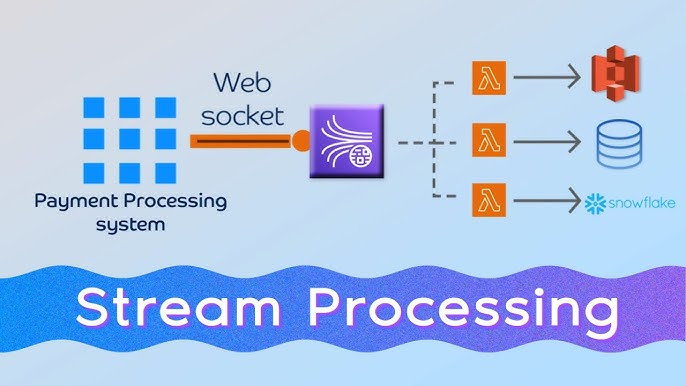
\includegraphics[width=.6\textwidth]{Streaming.jpg}
    \label{fig:my_label}
\end{figure}

\subsection{Ejemplos}

El sistema de procesamiento de secuencias resulta beneficioso en la mayoría de las situaciones en las que se generan datos nuevos y dinámicos
de forma continua. Aplica a la mayoría de los sectores y casos de uso de macrodatos:
\begin{itemize}
    \item Monitorización de sistemas, de redes y de aplicaciones
    \item Dispositivos Internet of Things (IoT)
    \item Sistemas de recomendación y optimización de resultados
    \item Transacciones financieras, detección de fraude y trading
    \item Multimedia y videojuegos
    \item Seguimiento de usuarios en páginas web y comercio electrónico
    \item Notificaciones en dispositivos y aplicaciones móviles en tiempo real
\end{itemize}

\subsection{Ventajas}

\begin{itemize}
    \item \textbf{Procesamiento en tiempo real}\\
    Como hemos descrito antes, el procesamiento en streaming permite analizar y actuar sobre los datos en tiempo real.
    \item \textbf{desacoplamiento}\\
    Por ejemplo en una arquitectura editor-subscriptor, el editor no necesita saber quién está suscrito a sus mensajes, 
    y los subscriptores no necesitan saber quién es el editor. Esto permite una mayor flexibilidad y escalabilidad.
    \item \textbf{Independencia}\\
    Esto es posible gracias al desacomplamiento Los equipos no necesitan una gran coordinación para trabajar en cada uno 
    de los extremos. También, las tecnologías de streaming nos facilitan implementar una arquitectura de microservicios.
\end{itemize}

\subsection{Desventajas}

\begin{itemize}
    \item \textbf{Coste elevado}\\
    El coste de implementación y mantenimiento de un sistema de procesamiento en streaming puede ser más elevado que
    el procesamiento en batch. Además de requerir un nivel de conocimientos adecuado.
    \item \textbf{Latencia}\\
    A pesar de ser un procesamiento casi inmediato, puede llegar a generar más retraso en algunos momentos de lo que
    se espera. Esto puede ser un problema en aplicaciones que requieran una respuesta inmediata.
\end{itemize}

\clearpage

\section{Procesamiento en tiempo real}

\subsection{Definición}

El sistema de procesamiento en tiempo real se refiere a aquellos que el análisis y la respuesta es inmediata a los datos conforme se
reciben, sin demora alguna.
\\
A diferencia del procesamiento en streaming, en este no hay ningún tipo de latencia y se procesa cada evento al momento.

\begin{figure}[h!]
    \centering
    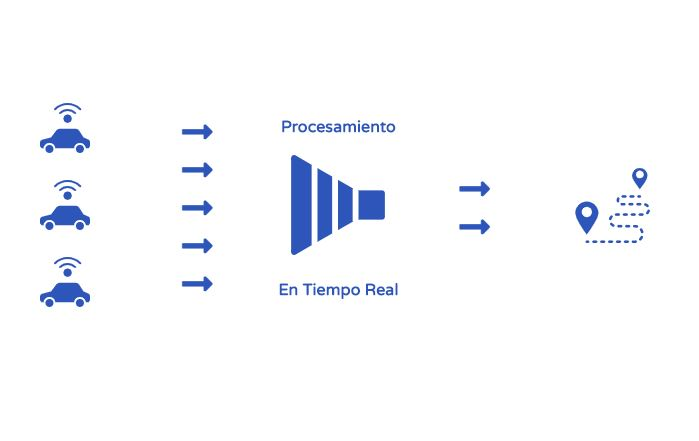
\includegraphics[width=.6\textwidth]{TiempoReal.jpg}
    \label{fig:my_label}
\end{figure}

\subsection{Ejemplos}

\begin{itemize}
    \item \textbf{Movimiento de datos en tiempo real}\\
    transmisión de datos desde cientos de miles de dispositivos y la realización de transformaciones ETL en grandes volúmenes de datos 
    continuos y de alta velocidad en tiempo real permiten a los usuarios analizar los datos tan pronto como se producen.
    \item \textbf{Análisis de datos en tiempo real}\\
    Analice los datos tan pronto como se generen y permita tomar decisiones en tiempo real en toda la organización para aprovechar las 
    oportunidades, mejorar las experiencias de los clientes, evitar fallos en las redes o actualizar las métricas empresariales críticas en 
    tiempo real.
    \item \textbf{Procesamiento de transmisiones de eventos}\\
    Capture y responda a los eventos a medida que ocurren en tiempo real en varias aplicaciones. Los casos de uso más comunes son la 
    comunicación entre cientos de microservicios desacoplados y el mantenimiento de un sistema de registro mediante Change Data Capture. 
\end{itemize}

En todos estos ejemplos es fundamental que la latencia sea minima porque este enfoque se basa en la capacidad de reaccionar y tomar decisiones 
instantáneamente.

\subsection{Comparación}

\begin{itemize}
    \item \textbf{Latencia:}\\
    El streaming tiene baja latencia; el tiempo real busca latencia mínima o nula.
    \item \textbf{Frecuencia:}\\
    El streaming procesa datos en pequeños lotes; el tiempo real procesa cada evento de forma instantánea.
    \item \textbf{Requerimientos:}\\
    El streaming puede tolerar ligeros retrasos; el tiempo real exige alta capacidad de respuesta y precisión inmediata.
\end{itemize}

\clearpage
\section{Comparativa entre los tres tipos de procesamiento}

\renewcommand{\arraystretch}{2} % Espaciado vertical en las celdas

\begin{tabularx}{\textwidth}{|>{\raggedright\arraybackslash}X|>{\raggedright\arraybackslash}X|>{\raggedright\arraybackslash}X|>{\raggedright\arraybackslash}X|}
    \hline
    \textbf{Tipo} & \textbf{Procesamiento por Lotes} & \textbf{Procesamiento en Streaming} & \textbf{Procesamiento en Tiempo Real} \\
    \hline
    \textbf{Latencia} & Alta (puede tardar minutos, horas o más). & Media (procesa datos casi en tiempo real, pero con un pequeño retraso) & Muy baja (milisegundos o menos) \\
    \hline
    \textbf{Frecuencia de actualización} & Periódica (procesos programados) & Continua (procesa datos a medida que llegan) & Instantánea (procesa cada evento al momento)\\
    \hline
    \textbf{Volumen de datos} & Grandes volúmenes procesados en conjunto & Flujo constante de datos & Flujo constante de datos \\
    \hline
    \textbf{Aplicaciones recomendadas} & -Generación de informes -Investigación Médica  -Tareas programables & -Análisis de datos en tiempo casi real -Detección de anomalías -Transmisiones en vivo & -Vigilancia de fraudes -Control de maquinaria -Juegos interactivos \\
    \hline
    \textbf{Ventajas} & -Eficiencia en el uso de recursos -Procesar grandes cantidades de datos & -Proporciona resultados en tiempo cercano al real -Manejo continuo de datos & -Respuesta inmediata -Ideal para decisiones críticas \\
    \hline
    \textbf{Limitaciones} & -No apto para aplicaciones sensibles al tiempo -Retraso entre la recopilación y el análisis de datos &  -Requiere más recursos que el procesamiento por lotes -Puede tener mayor latencia que el tiempo real & -Complejidad técnica -Alto costo de implementación y mantenimiento \\
    \hline
\end{tabularx}

\clearpage

\section{Conclusión}

Como hemos visto, cada uno de los tres tipos de procesamiento de datos en Big Data tiene sus propias ventajas y desventajas.
Dependiendo de las necesidades de la empresa, se deberá de elegir uno u otro. Si se requiere de un procesamiento de grandes volumenes
de datos y no se necesita una respuesta inmediata, el procesamiento por lotes es la mejor opción. Si se necesita una respuesta casi inmediata
y se puede tolerar un pequeño retraso, el procesamiento en streaming es la mejor opción. Por último, si se necesita una respuesta inmediata
y no se puede tolerar ningún tipo de retraso, el procesamiento en tiempo real es la mejor opción.

\clearpage

\section{Bibliografia}

\cite{aws_batch_processing}
\cite{aws_real_time_streaming}
\cite{aws_streaming_data}
\cite{appmaster_real_time_processing}
\cite{confluent_data_streaming}
\cite{aprenderbigdata_stream_processing}
\cite{foqum_real_time_processing}
\cite{powerdata_real_time_advantages}
\cite{profesionalreview_batch}
\cite{wikipedia_lotes}

\printbibliography

\end{document}
